\documentclass{article}

\usepackage[preprint]{nips_2018}
\usepackage[utf8]{inputenc}
\usepackage[T1]{fontenc}
\usepackage{hyperref}
\usepackage{url}
\usepackage{booktabs}
\usepackage{amsfonts}
\usepackage{nicefrac}
\usepackage{microtype}
\usepackage{amsmath}
\usepackage{algorithm}
\usepackage{algorithmicx}
\usepackage{algpseudocode}
\usepackage{ctex}
% \usepackage{palatino}
\usepackage{tikz}
\usetikzlibrary{shapes.geometric, arrows}
\title{深度神经网络求解偏微分方程}

\author{
  肖新宇\\数学科学学院\\北京大学\\ \texttt{2001110035} \\
}

\begin{document}

\maketitle

\begin{abstract}
\par 经典的偏微分方程求解方法包括有限差分,有限元,谱方法等。这些方法基本上都需要生成网格,而在复杂的区域或者高维问题上,这种网格方法由于维数灾难而失效。近年来,随着深度学习的兴起,一种利用深度神经网络(DNN)逼近解的无网格方法\cite{PINN}也崭露头角。为了验证这种方法的有效性,在这篇报告中利用DNN成功求解了泊松方程(不含时的情况),Burgers方程(含时非线性)。在泊松方程的例子中,我采取了一种改进方法避免边界惩罚项获得了比原始方案更精确的解。在含时的Burgers方程的例子中,我将NN(Neural Network)的近似解与经典的傅里叶谱方法的高精度解作为对比。发现在求解非含时和含时方程时,DNN方法都得到了不错的结果。
\end{abstract}

\section{引言}
深度学习\cite{lecun2015deep}在图像的分类、目标检测等许多任务上都取得了最好的结果,近年来迅速来应用到各个科学与计算领域。这得益于其良好的逼近能力、灵活性和解决维度灾难的能力。人们很自然地会想到一种合适的方法来使用深度学习来求解偏微分方程。 \cite{yu2017deep} 提出了一种通过神经网络逼近解的方法,并使用Ritz方法来解决泊松型方程。\cite{DGM}\cite{PINN}使用了平方误差损失函数(DGM:Deep Garlerkin Method)解含时方程。 \cite{1707.02568}\cite{weinan2017deep}\cite{beck2017machine} 则首先将偏微分方程转化为后向随机微分方程,然后使用神经网络或其他机器学习方法来逼近它们的解。


\par 在本报告中,我们重点关注的是 Deep Galerkin 方法 \cite{PINN}。本报告的内容组织如下:
\begin{itemize}
\item 在第2节中,介绍了DNN求解PDE的思路,并简要推导了该算法的理论,给出了一个启发性的解释.
\item 在第3节中使用DNN方法求解了Poisson方程,并对该算法提出了一个避免惩罚项的改进,得到了更精确的解。
\item 在第4节中使用DNN方法求解了Burgers方程,并将其结果与经典的傅里叶谱方法结果进行了对比。
\item 在第5节中总结了这种方法的优点和缺点,并对未来的研究方向做了一些展望。
\end{itemize}

\section{Deep Galerkin Method}
考虑一个含时或者不含时的偏微分方程初边值问题(不含时的情况就去掉下面公式中的$\partial_t$):
\begin{equation}
\left\{\begin{array}{ll}\left(\partial_{t}+\mathcal{L}\right) u(t, \boldsymbol{x})=0, & (t, \boldsymbol{x}) \in[0, T] \times \Omega \\ u(0, \boldsymbol{x})=u_{0}(\boldsymbol{x}), & \boldsymbol{x} \in \Omega \\ u(t, \boldsymbol{x})=g(t, \boldsymbol{x}), & (t, \boldsymbol{x}) \in[0, T] \times \partial \Omega\end{array}\right.
\end{equation}
使用一个神经网络逼近解函数:
\begin{equation}\label{approximation}
u(x,t) \approx \hat{u}(x,t,\theta)
\end{equation}
构建DGM损失函数:
\begin{equation}\label{DGM loss}
\begin{array}{l}
J(\theta)=\operatorname{loss}_{1}+\operatorname{loss}_{2}+\operatorname{loss}_{3}\\
\operatorname{loss}_{1}=\left\|\frac{\partial \hat{u}}{\partial t}(t, x ; \theta)+\mathcal{L} \hat{u}(t, x ; \theta)\right\|_{[0, T] \times \Omega, \nu_{1}}^{2}\\
\operatorname{loss}_{2}=\|\hat{u}(t, x ; \theta)-g(t, x)\|_{[0, T] \times \partial \Omega, \nu_{2}}^{2}\\
\operatorname{loss}_{3}=\left\|\hat{u}(0, x ; \theta)-u_{0}(x)\right\|_{\Omega, \nu_{3}}^{2}
\end{array}
\end{equation}
$loss_1$代表内部方程的损失项,强制要求神经网络拟合的函数在区域内部满足方程(在使用了Monta Carlo采样后,即要求方程在某些配点上成立)。$loss_2$e和$loss_3$分别为边界惩罚项,初始条件惩罚项,强制要求$\hat{u}(x,t,\theta)$满足初边值条件。\\
我们的目标是求解$\hat{u}(x,t,\theta)$使得损失函数极小:
\begin{equation}\label{minimize}
	\begin{cases}
 		\text{Find} \ \hat{u} \in H& x\in \Omega, \\
 		minimize \ I(\hat{u})
 	\end{cases}
\end{equation}
下面考虑Poisson方程这个损失函数下的变分方程以说明Poisson方程的解是\ref{DGM loss}的唯一极值点,(对Burgers方程的变分形式没有推出类似结果,只能说明Burgers方程的解是一个极小点,不能保证唯一性)。
\subsection{Poisson equation变分方程推导}
考虑泊松方程DGM损失函数的变分:
\begin{align*}
I(u) &= \int_{\Omega} \|\Delta u + f\|^2 dx + \int_{\partial \Omega} \|u-g\|^2ds \\
\delta I &= 2\int_{\Omega}(\Delta u + f)\Delta (\delta u) dx + 2\int_{\partial \Omega}(u-g)\delta u \ ds
\end{align*}
令$v = \Delta u + f$,并利用Green第二等式可知:
\begin{align*}
\delta I &= 2\int_{\Omega}\Delta(v)\delta u\ dx + 2\int_{\partial \Omega}\left[v\frac{\partial \delta u}{\partial n} + (u-g -\frac{\partial v}{\partial n})\delta u \right] ds
\end{align*}
若该变分方程对任意$\delta u$都成立,则可知
\begin{equation}\label{eq1}
	\begin{cases}
 		\Delta v=0, & x\in \Omega, \\
 		v=0, & x\in \partial \Omega. \\
 		u=g+\frac{\partial v}{\partial n}, & x\in \partial\Omega.
 	\end{cases}
\end{equation}
由\ref{eq1}的前两式可知$v = 0$,所以可以推出:
\begin{equation}\label{Poisson}
	\begin{cases}
 		-\Delta u = f,& x\in\Omega \\
 		u=g, & x\in \partial\Omega.
 	\end{cases}
\end{equation}
这就说明该变分方程的解就是Poisson方程的解。也就说明了Poisson方程是DGM损失函数的唯一极值点。

\subsection{DNN网络结构}
\par{} 在构建PDE解的逼近函数\ref{approximation}时,使用的Deep-learning中常用的的Res-Net\cite{ResNet}结构。
\begin{align*}\label{res_equ}
	s_1 &= \phi(W_1 x_0 + b_0) \\
	s_i &= \phi(W_{i2}\cdot\phi(W_{i1}\cdot s_{i_1}+b_{i1})+b_{i2})+s_{i-1}, (2\leq i \leq N-1)\\
	s_N &= W_N\cdot s_{N-1} + b_N
\end{align*}
其中$s_{i}$是神经网络第i层的输出, $W_{i1},W_{i2}\in R^{m\times m},b_{i1},b_{i2}\in R^{m}$ 为中间层的参数。N为网络的深度,m为网络的宽度,这两个参数限制神经网络的规模。$\phi$ 是激活函数,在我们的应用中,将取为
$$
\phi(x) = \tanh(x) = \frac{e^{x} - e^{-x}}{e^x + e^{-x}}
$$
这种取法是论文\cite{PINN}的做法。网络结构示意图可以参见\ref{architecture}。
\begin{figure}[htbp]
	\centering
	\setlength{\belowcaptionskip}{10pt}
	\caption{Network Structure of Deep Galerkin method}
	\label{architecture}
	\tikzstyle{startstop} = [rectangle, rounded corners, minimum width = 2cm, minimum height=1cm,text centered, draw = black, fill=red]
	\tikzstyle{io} = [trapezium, trapezium left angle=80, rounded corners = 2mm, trapezium right angle=100, minimum width=2cm, minimum height=1cm, text centered, draw=black, fill=purple!50]
	\tikzstyle{process} = [rectangle, rounded corners = 2mm, minimum width=3cm, minimum height=0.5cm, text centered, draw=black, fill=pink!50]
	\tikzstyle{decision} = [diamond, aspect = 3, text centered, draw=black, fill=blue!30, align = center]
	\tikzstyle{add} = [rectangle, minimum size=6mm, rounded corners=3mm, very thick, draw=black!50, top color=white, bottom color=black!20]
	% 箭头形式
	\tikzstyle{arrow} = [->,>=stealth]
	\begin{tikzpicture}[node distance = 1cm]
	%定义流程图具体形状
	\node[io,  yshift = -1cm](in1){Input};
	\node(fc11) [process, below of = in1, yshift = -0.3cm]{FC layer(size m)};
	\node(fc12) [process, below of = fc11]{Activate};
	\node(add1) [add, below of = fc12]{+};
	\node(fc21) [process, below of = add1]{FC layer(size m)};
	\node(fc22) [process, below of = fc21]{Activate};
	\node(add2) [add, below of = fc22]{+};
	\node(fc31) [process, below of = add2]{FC layer(size m)};
	\node(fc32) [process, below of = fc31]{Activate};
	\node(add3) [add, below of = fc32]{+};
	\node(residual 1) [decision, right of = fc11, xshift = 5cm, yshift= -0.5cm]{Residue\\Connection};
	\node(residual 2) [decision, right of = fc21, xshift = 5cm, yshift= -0.5cm]{Residue\\Connection};
	\node(residual 3) [decision, right of = fc31, xshift = 5cm, yshift= -0.5cm]{Residue\\Connection};
	\node(fc4) [process, below of = add3]{FC layer(size 1) };
	\node(out1) [io, below of = fc4, yshift = -0.3cm]{Output};
	%连接具体形状
	\draw [arrow] (in1) -- (fc11);
	\draw [arrow] (0, -1.8) -| node  [right] {} (residual 1);
	\draw [arrow] (fc11) -- (fc12);
	\draw [arrow] (fc12) -- (add1);
	\draw [arrow] (residual 1) |- node [right] {} (add1);
	\draw [arrow] (add1) -- (fc21);
	\draw [arrow] (0, -4.8) -| node  [right] {} (residual 2);
	\draw [arrow] (fc21) -- (fc22);
	\draw [arrow] (fc22) -- (add2);
	\draw [arrow] (residual 2) |- node [right] {} (add2);
	\draw [arrow] (add2) -- (fc31);
	\draw [arrow] (0, -7.8) -| node  [right] {} (residual 3);
	\draw [arrow] (fc31) -- (fc32);
	\draw [arrow] (fc32) -- (add3);
	\draw [arrow] (residual 3) |- node [right] {} (add3);
	\draw [arrow] (add3) -- (fc4);
	\draw [arrow] (fc4) -- (out1);
	\end{tikzpicture}
\end{figure}

\subsection{Monta carlo积分近似}
由于积分表达式\ref{DGM loss}无法解析求出,所以这里需要采用数值积分的办法。在这里我们采用了一般的蒙特卡洛积分法:
$$
\int_{\Omega} f(x) \approx \frac{1}{N}\sum_{i=1}^{N} f(x_i)
$$
其中$x_i \sim Uniform(\Omega)$.采用这一技巧之后,若定义$f(x,t) = u_t(x,t;\theta) + \mathcal{L}u(x,t;\theta)$我们的损失函数可以变为:
\begin{align*}
MSE &= MSE_f + MSE_b + MSE_0 \\
&=\frac{1}{N_f}\sum_{i=1}^{N_f}\|f(x_f^i,t_f^i)^2\|^2 + \frac{1}{N_b}\sum_{i=1}^{N_b} \|u(x_b^i,t_b^i) - g(x_b^i,t_b^i)\|_2^2 + \frac{1}{N_0}\sum_{i=1}^{N_0} \|u(x_0^i,t_0^i) - u_0(x_0^i,t_0^i)\|_2^2
\end{align*}
其中第一项在区域$\Omega\times [0,T]$上均匀采样,第二项在边界上采样,第三项在初始时刻采样,实在训练中往往可以给三个项中做加权求和。
 \subsection{优化算法}
这在深度学习中经常使用的优化算法是以Adam为典型的随机梯度下降算法,但是在求解PDE时,我们往往需要更高的计算精度。在实验中我发现使用Adam等梯度算法不能得到令人满意的解,能工作的优化器是L-BFGS(有限内存的BFGS方法)。这是一种拟牛顿型的全梯度优化算法,也可以看成共轭梯度法的推广。更多的细节可以参考论文\cite{LBFGS},在pytorch的optim类中实现了这一类的优化器,可以直接调用。

\section{求解Poisson方程}
2D Poisson方程的Dirichlet边值问题,$\Omega = [-1,1]\times [-1,1]$
\begin{equation}
	\begin{cases}
 		-\Delta u=f(x), & x\in \Omega, \\
 		u=g(x), & x\in \partial \Omega, \\
 	\end{cases}
\end{equation}
采用2.2中提到的网络结构深度$N = 4$, 宽度$m = 20$, 损失函数在内部采样数为$N_f = 1000$,边界采样数$N_b = 100$.
损失的调配参数$\beta=10$.
$$
loss = MSE_f + \beta\cdot MSE_b
$$
\subsection{example 1}
我们人工构造出一个在边界和区域内部变化都比较复杂的测试函数如下:
$$
u_{real} = exp(x^2 + y^2)\cdot \sin(5x-2y) + xy,\ f(x,y) = -\Delta u_{real}, \ g(x,y)=u_{real}|_{\partial \Omega}(x,y)
$$
\begin{figure}[ht]
 	 \centering
 	 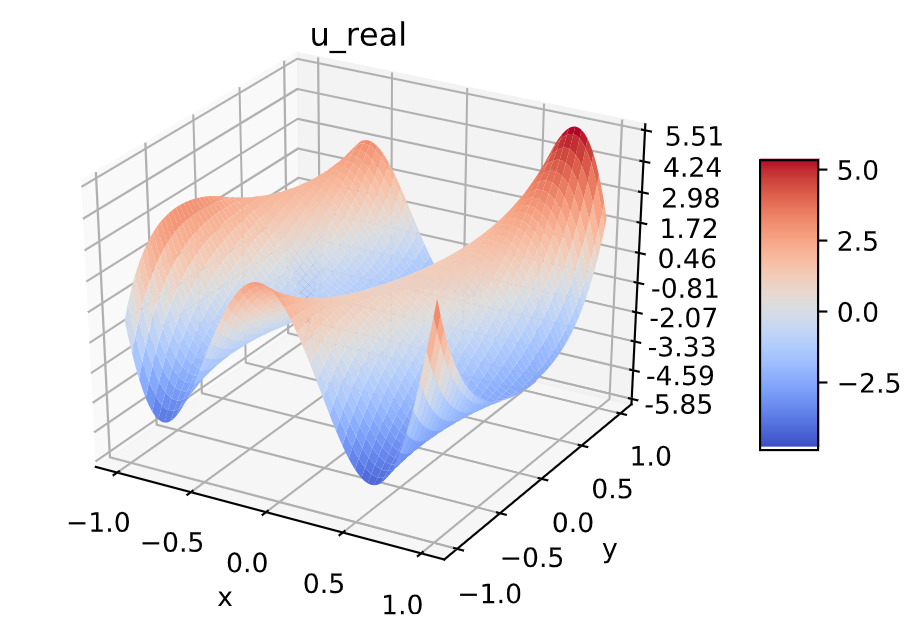
\includegraphics[width=0.45\textwidth]{images/poisson_real.png}
 	 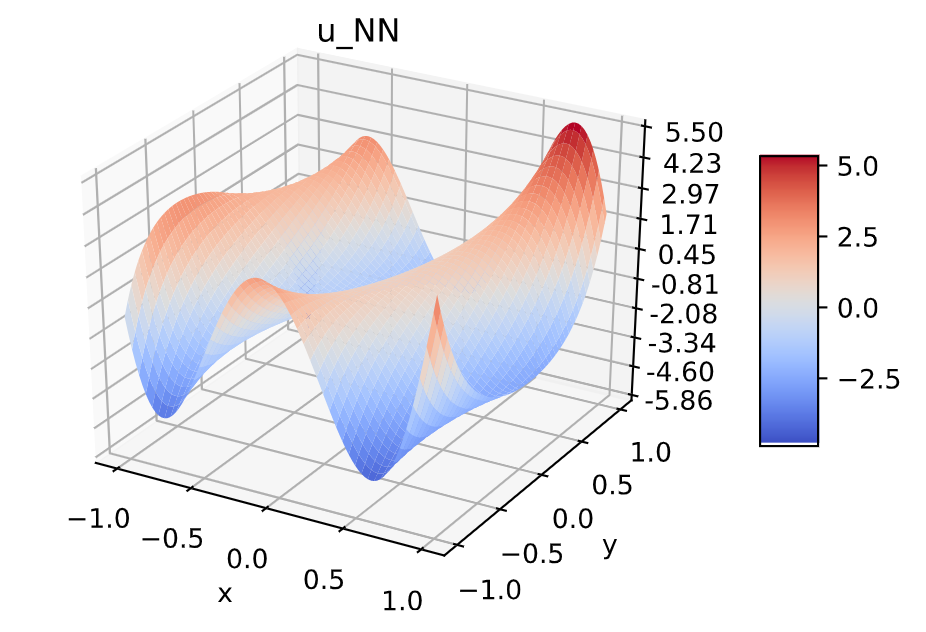
\includegraphics[width=0.45\textwidth]{images/poisson_NN.png}
	 \caption {泊松方程的解.左边: 真解, 右边: 神经网络近似解}
	 \label{解景观}
\end{figure}

\begin{figure}[ht]
 	 \centering
 	 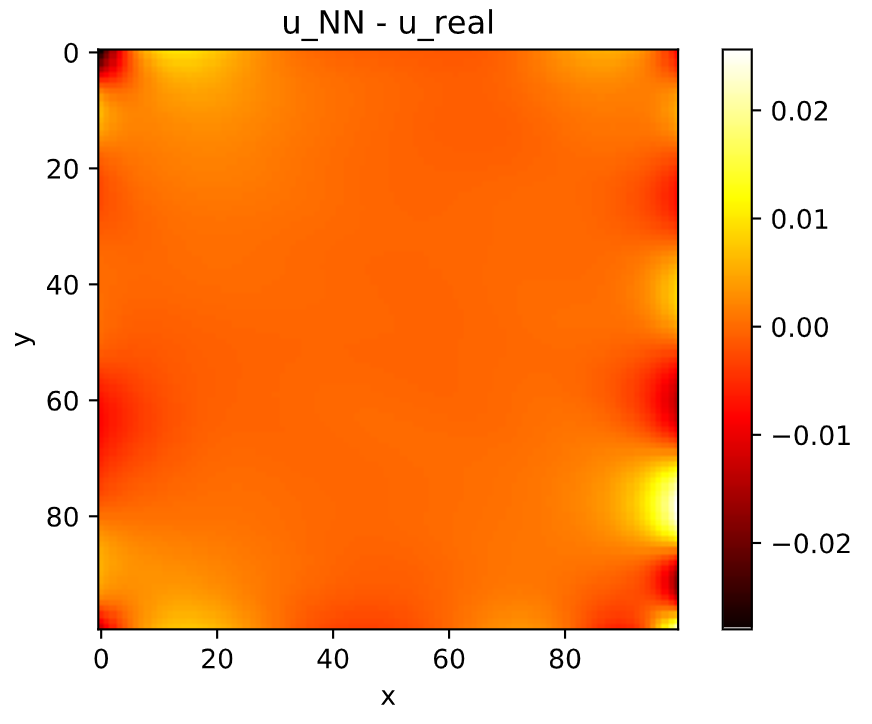
\includegraphics[width=0.4\textwidth]{images/poisson_error.png}
 	 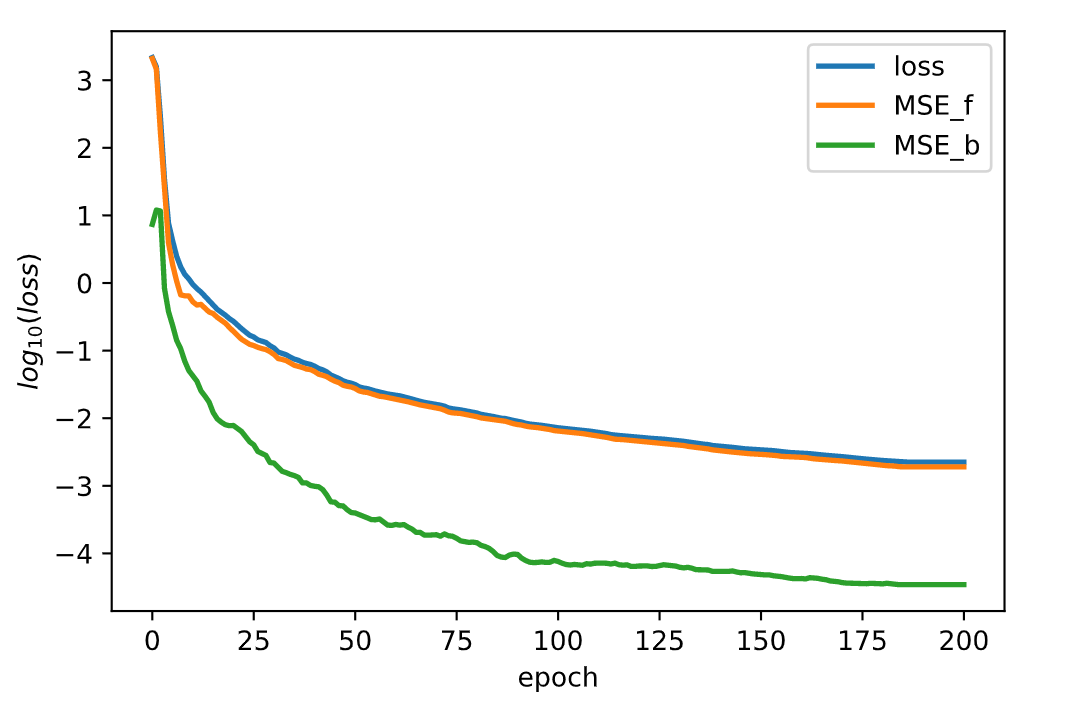
\includegraphics[width=0.5\textwidth]{images/poisson_loss.png}
	 \caption {左边:误差图 $u_{real} - u_{NN}$ 右边:损失函数下降曲线图}
	 \label{误差图和Loss图}
\end{figure}

\begin{table}[ht]
\centering  
\caption{Relative Loss of Different $\beta$ with Poisson Equation: error定义见\ref{relative L2 error}}
\label{比较不同系数}
\begin{tabular}{ccc} 
	\toprule
	$\beta$ & Relative Loss (\%) \\
	\hline
	10 & 0.33 \\
	\hline
	100 & 0.19 \\
	\hline
	1000 & 0.48 \\
	\bottomrule
\end{tabular}
\end{table}

\begin{equation}\label{relative L2 error}
error =  \left(\int_{\Omega}\left(u^{*}\left(x ; \theta^{*}\right)-u(x)\right)^{2} \mathrm{~d} x\right)^{\frac{1}{2}} \cdot\left(\int_{\Omega}(u(x))^{2} \mathrm{~d} x\right)^{-\frac{1}{2}}
\end{equation}

从图\ref{解景观}可以看到,我们得到的近似解确实和真解呈现出相同的图景,这意味着我们得到了正确的解。从\ref{误差图和Loss图}左边的误差图可以看出,拟合得不太好的地方主要分布在区域的边界附近。于是我增大了$\beta$到100,使得边界项的损失具有更大的比重,发现结果确实变得更好(如表\ref{比较不同系数}所示)。但是当我继续增大$\beta$到1000,结果反而变差。其原因可能是,
\begin{itemize}
\item 1.这是一个内部误差与边界误差进行权衡的问题,过大的$\beta$使得内部误差项被忽略。
\item 2.过大的$\beta$使得问题变得奇异,难以优化。
\end{itemize}
下一小节我们便来解决这个问题:
\subsection{Penalty free的改进方案}
这一小节要解决上一节中$\beta$的选取问题。我们采取有一种更加直接的方式避免这个调参问题:将我们的试验函数直接构造在满足边界条件的函数空间如下
$$
u(x,\theta) = l(x)\cdot v(x,\theta) + \tilde{g}(x)
$$
其中$v(x,\theta)$是一个神经网络,$l(x)$是一个到边界的距离函数,比如在我们这个例子中可以取$l(x,y) = (1-x^2)(1-y^2)$,而$\tilde{g}(x)$是边界函数$g(x)|_{\partial \Omega}$的延拓,.但是问题在于如何得到$g(x)$的延拓呢?如果我们直接让$\tilde{g}(x) = u_{real}(x)$那么这当然存在作弊的嫌疑,因为我们是事先是不知道真解的。想法是使用另一个小型的神经网络$h(x,\theta_1)$拟合$\tilde{g}(x)$.这样,我们的算法可以拆分为两个独立的优化问题,描述如下:
\begin{itemize}
\item 第一步: 优化边界损失函数
\begin{equation}\label{partial loss}
\theta_1 = \mathop{argmin}\limits_{\theta_1} MSE_b(\theta_1) = \frac{1}{N_b}\sum_{i=1}^{N_b} \|h(x_i,\theta_1)-g(x_i)\|^2
\end{equation}
\item 第二步:构建试验函数:
\begin{equation}\label{new trial fun}
u(x,\theta) = l(x)\cdot v(x,\theta) + h(x,\theta_1)
\end{equation}
\item 第三步:优化内部损失函数
\begin{equation}\label{int loss}
\theta = \mathop{argmin}\limits_{\theta} MSE_f(\theta) = \frac{1}{N_f}\sum_{i=1}^{N_f} \|f(x_f^i,\theta)\|^2
\end{equation}
其中$f = \Delta u(x,\theta) + f$。
\end{itemize}
按照上面的方案进行求解,遗憾的是,并没有达到解得更好的结果,这是什么原因呢?将$h(x,\theta_1)$的图像画出来(如图\ref{h_NN}左)可以知道h虽然拟合好了边界,但是内部延拓出来的解由于没有任何束缚而离真解非常远,甚至奇异,这毫无疑问大大提高了第二步优化的难度。所以我们应当对$h$内部加适当的约束。这个约束就不妨直接取为求解方程的内部MSE,这样\ref{partial loss}就可以改进为\ref{new partial loss}.
\begin{figure}[ht]
\centering
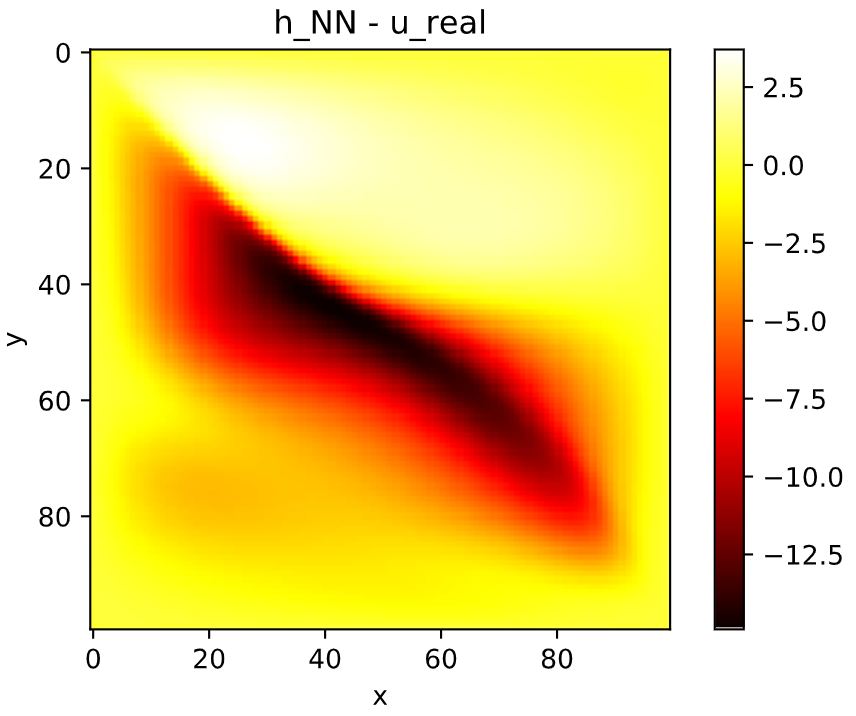
\includegraphics[width=0.45\linewidth]{images/h_NN_old.png}
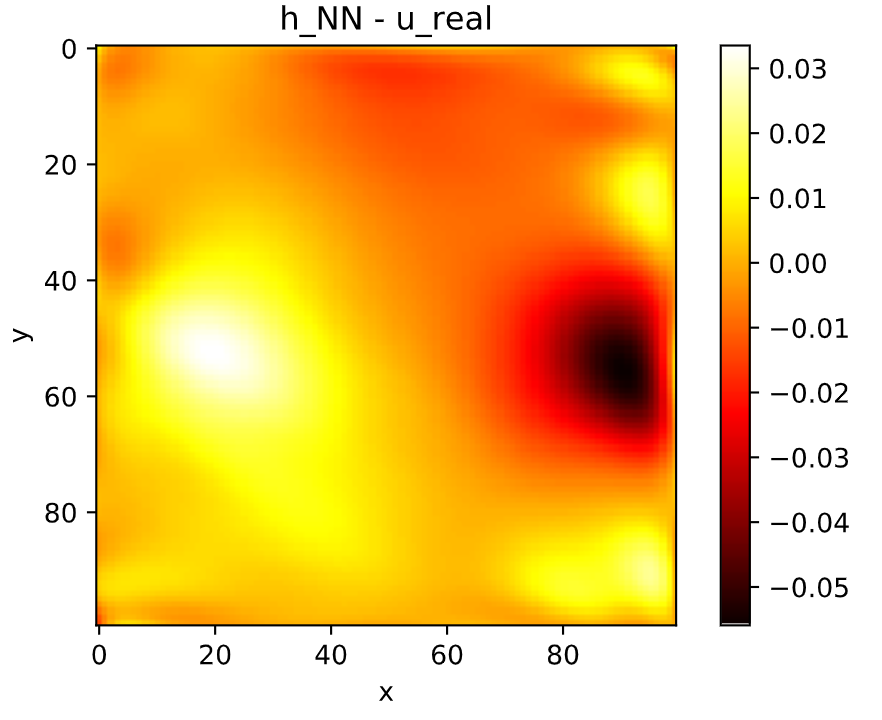
\includegraphics[width=0.45\linewidth]{images/h_NN_new.png}
\caption{左图:使用\ref{partial loss}的$h$与真解的误差(没有采用正则项), 右图:使用\ref{new partial loss}的$h$与真解的误差(采用了正则项).可以看到是用了正则项后的h与真解已经很接近了,这会大大降低第二步优化的难度.}
\label{h_NN}
\end{figure}
\begin{equation}\label{new partial loss}
\theta_1 = \mathop{argmin}\limits_{\theta_1} \beta MSE_b(\theta_1) + MSE_f(\theta_1)= \frac{\beta}{N_b}\sum_{i=1}^{N_b} \|h(x_i,\theta_1)-g(x_i)\|^2 + \frac{1}{N_f}\sum_{i=1}^{N_b} \|f(x_f^i,\theta_1)\|^2
\end{equation}
在式\ref{new partial loss}中,第二项为正则项,这一项的存在使得$h(x,\theta_1)$内部大致和真解相同(这样我们第二步优化\ref{int loss}中的$v(x,\theta)$将接近与0函数,这是与神经网络参数零初始化相匹配的)。 然后,我们取$N_f = 100$(内部点), $N_b=1000$(边界点), $\beta=1000$,保证第一步优化精确地拟合边界函数。综合起来使用\ref{new partial loss},\ref{new trial fun},\ref{int loss},并且设置参数如表\ref{参数配置},最终的结果对比如表\ref{改进 vs 不改进}。
\begin{table}[ht]
\centering  
\caption{分步优化的参数设置}
\label{参数配置}
\begin{tabular}{ccccccc} 
	\toprule
	步骤 & 优化对象         & 网络宽度 &  网络深度 &   $\beta$ & $N_f$(内部取样) & $N_b$(边界取样)\\
	\hline
	1   &$h(x,\theta_1)$ & 20 &  3   & 1000 & 1000 & 100 \\
	\hline
	2   & $v(x,\theta)$   & 30 & 4  & 0   & 0     & 1000\\
	\hline
	\bottomrule
\end{tabular}
\end{table}

\begin{table}[ht]
\centering  
\caption{改进结果对比}
\label{改进 vs 不改进}
\begin{tabular}{cc} 
	\toprule
	项 & Relative Loss (\%) \\
	\hline
	\hline
	原始形式($\beta=100$) & 0.19 \\
	\hline
	改进分步优化 & 0.15 \\
	\bottomrule
\end{tabular}
\end{table}

\section{求解Burgers方程}
\begin{equation}\label{burgers}
	\begin{cases}
 		u_{t}+u u_{x}-\nu u_{x x}=0, \quad x \in[-1,1], \quad t \in[0,1], \\
		u(0, x)=-\sin (\pi x) \\
		u(t,-1)=u(t, 1)=0
 	\end{cases}
\end{equation}
这个方程的真解在文章\cite{spectral}给出了:
$$
u(x, t)=4 \pi \nu\left[\sum_{n=1}^{\infty} n a_{n} \mathrm{e}^{-n^{2} \pi^{2} t \nu} \sin n \pi x \Big/\left(a_{o}+2 \sum_{n=1}^{\infty} a_{n} \mathrm{e}^{-n^{2} \pi^{2} t \nu} \cos n \pi x\right)\right]
$$
在我们的求解算例中令$\nu = 0.01 / \pi$, 内部采样数$N_f = 2000$, 边界采样数$N_b = 100$, 初始条件采样数$N_0 = 100$,
网络宽度$m = 30$, 深度$N=5$.求解结果如图\ref{BG}.
\begin{figure}[ht]
 	 \centering
 	 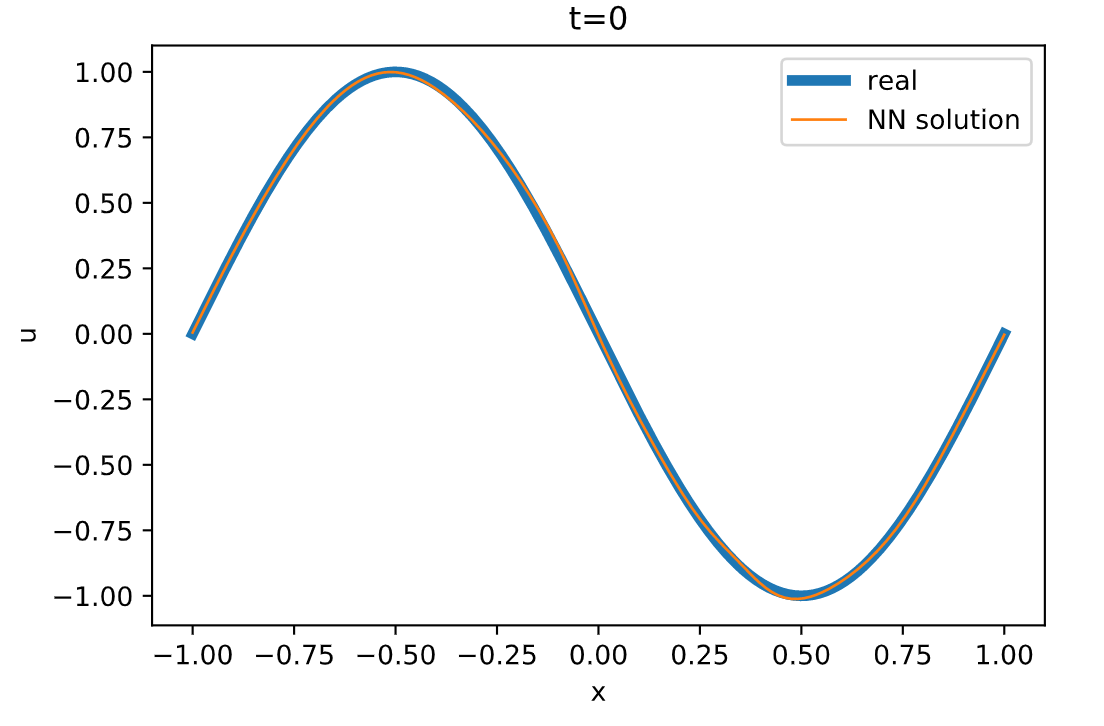
\includegraphics[width=0.45\textwidth]{images/BG_t0.png}
 	 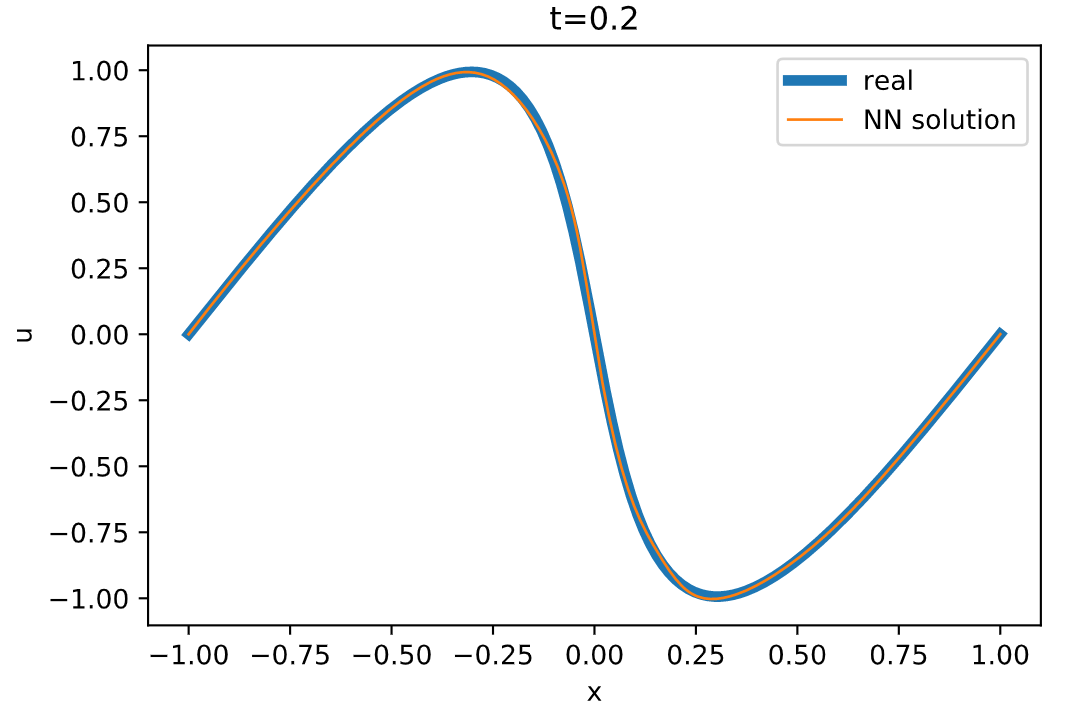
\includegraphics[width=0.45\textwidth]{images/BG_t1.png}

 	 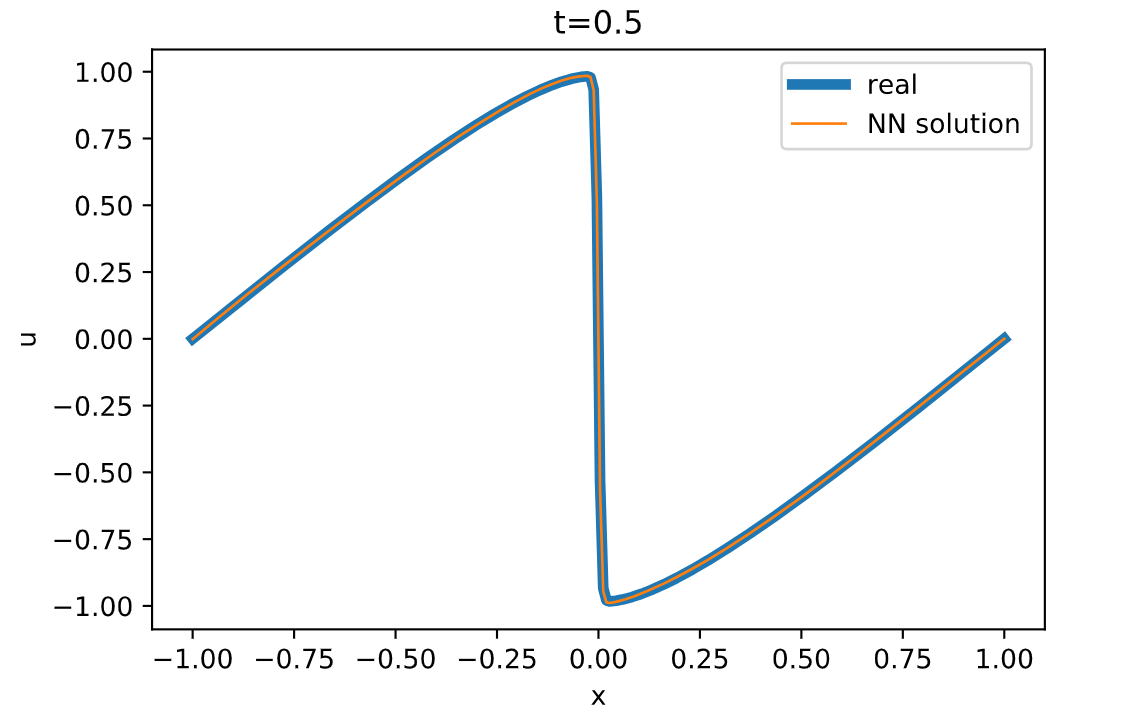
\includegraphics[width=0.45\textwidth]{images/BG_t2.png}
 	 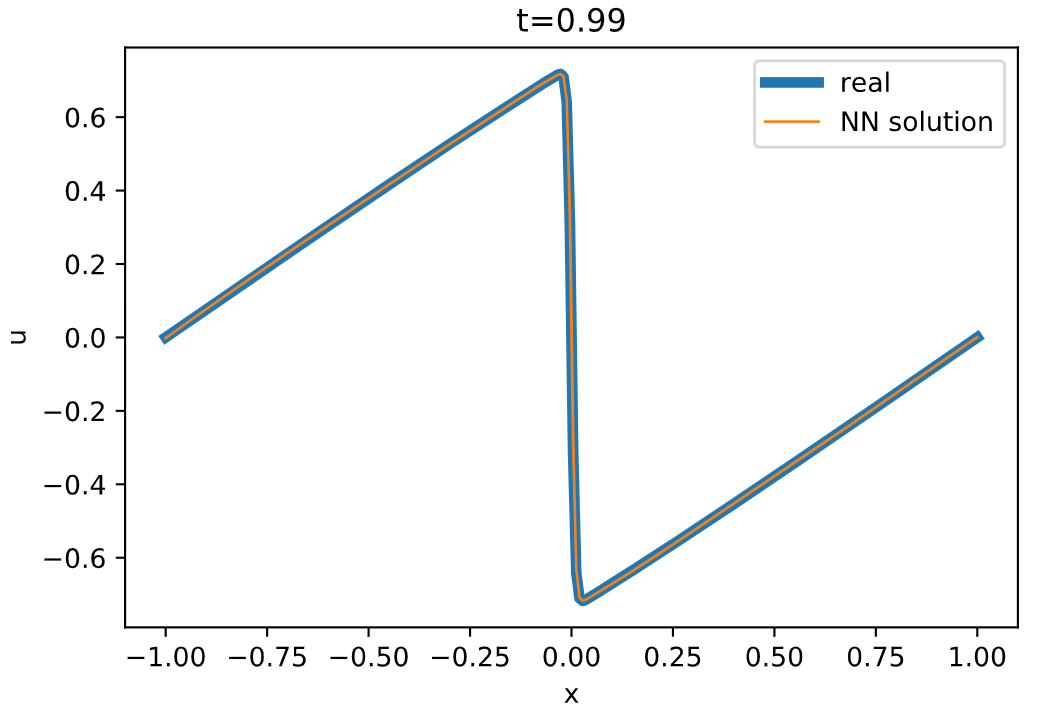
\includegraphics[width=0.45\textwidth]{images/BG_t3.png}
	 \caption {NN solution vs real solution,相对$L_2$误差为 $0.9\%$,相对$L_2$误差定义见\ref{relative L2 error}}
	 \label{BG}
\end{figure}
在表格\ref{Burgers结果对比}中展示了$N_f=1000$和$N_f=2000$的结果对比,发现提高内部采样数确实能够提高求解的精度。从图中结果也可以看出,DNN求解含时非线性方程时能够捕捉到激波结构,某种程度上证明这种方案是有效的。当然,真实的情况还需要更多的计算结果来支持和验证。
\begin{table}[ht]
\centering  
\caption{不同内部采样数的结果对比}
\label{Burgers结果对比}
\begin{tabular}{cc} 
	\toprule
	$N_f$ & Relative Loss (\%) \\
	\hline
	\hline
	1000 & 11  \\
	\hline
	2000 & 0.91 \\
	\bottomrule
\end{tabular}
\end{table}


\section{结论和展望}
在这篇报告中,我们使用PINN\cite{PINN}的深度神经网络方法求解了Poisson equation和Burgers euquation。验证了深度网络在求解PDE(含时,不含时)的有效性。在求解Poisson方程时,我给出了一种Penalty free的改进方案,避免了参数调节,并且得到了比原始方案更好的结果。在求解Burgers方程时,成功用DNN的方法捕捉了激波结构,验证了该方案在含时方程中的有效性。
\\
总结来说,深度网络求解PDE的优势在于mesh-free,而且依赖于神经网络强大的表达能力,能够拟合激波(比如burgers方程中的shock)。目前也已经有一系列的工作将这种方案应用于计算流体力学中,如\cite{NS-PINN}等,成功模拟了复杂的二维不可压流体的运动,由于时间所限制,报告的内容没有继续探索。DNN方案的缺点在于没有良好的收敛性保证定理,这也是一个非常困难而且值得研究的方向。

\section{附录}
文中所有的实验代码都是亲自实现的,并且已经和报告一起提交。由于上次课堂报告时实验部分尚未完全完成,所以并没有展示自己的实验结果,显得内容有些空洞。但是这个项目其实花费了我不少的时间和心血,只是在探索过程中发现不少想法可能早已被一些文章所发表,不得已在课堂报告中呈现出一种”综述“
的形式。希望这份期末报告能够让老师和助教看到我的一些思考和努力。
\bibliography{reference}
\bibliographystyle{plain}


\medskip

\small

\end{document}
